\documentclass[12pt,a4paper]{article}
\usepackage[utf8]{inputenc}
\usepackage{amsmath}
\usepackage{amsfonts}
\usepackage{amssymb}
\usepackage[french]{babel}
\usepackage{tikz}
\usepackage{placeins}
\usepackage{graphicx}
\usepackage{multirow}
\usepackage{hyperref}

\makeatletter
\newcommand*{\rom}[1]{\expandafter\@slowromancap\romannumeral #1@}
\makeatother

\setlength{\parskip}{1ex plus 0.5ex minus 0.2ex}
\newcommand{\hsp}{\hspace{20pt}}
\newcommand{\HRule}{\rule{\linewidth}{0.5mm}}
\newenvironment{remarque}{\textbf{Remarque :}}{}


\title{Cahier des charges}
\author{PaquiTeam}


\begin{document}

\begin{titlepage}
	\begin{center}
	
		
		\vfill
					
		\textsc{\LARGE PaquiTeam}\\[1.5cm]
		
		% Title
		\HRule \\[0.4cm]
			{ \huge \bfseries Présentation des cas d'utilisation principaux :\\
			Paquito, easy packaging\\[0.4cm]
			
\includegraphics[width=0.2\textwidth]{../img/paquito.png}
	
			}
		\HRule \\[1.5cm]
		% Author and supervisor
		
		\begin{minipage}{0.40\textwidth}
			\begin{flushleft} \large
				\emph{Auteurs :}\\
				Lucas \textsc{Robin}\\
				Kevin \textsc{Fleuriot}\\
				Alexandre \textsc{Noiret}\\
				Yassine \textsc{Ait Elmouden}\\
				Seynabou \textsc{Ka}
			\end{flushleft}
		\end{minipage}
		\hfill
		\begin{minipage}{0.40\textwidth}
			\begin{flushright} \large
				\emph{Clients :}\\
				Michael \textsc{Fortier}\\
				Hugues \textsc{Leprieur}
			\end{flushright}
		\end{minipage}

		\vfill			
		{\large 21 janvier 2016}
		\vfill
		\begin{minipage}{0.35\textwidth}
			\begin{flushleft}
				
\includegraphics[width=1\textwidth]{../img/UP13.png}			
			\end{flushleft}
		\end{minipage}
		\hfill
		\begin{minipage}{0.35\textwidth}
			\begin{flushright}
				
\includegraphics[width=1\textwidth]{../img/sup-galile.png}
			\end{flushright}
		\end{minipage}
		
									
	\end{center}		
\end{titlepage}

\section*{Introduction}
	De nos jours, tout le monde dispose d'un ordinateur à des fins personnelles ou professionnelles.
Les ordinateurs ont tous des architectures différentes (32 ou 64 bits) et des systèmes d'exploitation différents.

Dans le cas particulier de Linux, il existe même des distributions différentes comme Debian ou RedHat,...).

C'est là que notre problème se pose car si on prend Linux, il existe un logiciel qui est installé à travers un paquet récupéré sur le dépôt d'une distribution. Cependant, il peut y avoir des problèmes de compatibilité entre certaines distributions et le paquet du logiciel. Par conséquent, la personne ne pourra pas installer le paquet du logiciel directement sur sa machine et l'oblige à récupérer les sources du paquet et de devoir assurer la compilation. 

Le projet Paquito, qui a par ailleurs déjà été initié, permet de répondre à ce problème.

Nous allons vous présenter à travers différentes parties les solutions que l'on va proposer.

\section*{Quelques définitions}
	\begin{itemize}\renewcommand{\labelitemi}{$\bullet$}
		\item \textit{Paquet} : Archive (fichier compressé) comprenant les fichiers informatiques, les informations et procédures nécessaires à l'installation d'un logiciel sur un système d'exploitation .
		\item \textit{Compilation} : Travail réalisé par un compilateur qui consiste à transformer un code source lisible par un humain en un fichier binaire exécutable par une machine.
		\item \textit{Dépôt/Miroir de paquets} : Un dépôt est un stockage centralisé et organisé de paquets, en vue de leur distribution sur le réseau ou bien un endroit directement accessible aux utilisateurs.
		\item \textit{Docker} : Logiciel automatisant le déploiement d'applications dans des conteneurs logiciels et empaquetant une application et ses dépendances dans un conteneur virtuel, qui pourra être exécuté sur n'importe quel serveur Linux. Ceci permet d'étendre la flexibilité et la portabilité d’exécution d'une application, que ce soit sur la machine locale, un cloud privé ou public, une machine nue. 
		\item \textit{Container} : Un type de cloisonnement d'un système d'exploitation dans certains systèmes de virtualisation légers réutilisant le noyau et éventuellement les bibliothèques du système hôte.
		\item \textit{GitHub} : Service web d'hébergement et de gestion de développement de logiciels, utilisant le logiciel de gestion de versions Git. Le nom GitHub est composé du mot "git" faisant référence à un système de contrôle de version open-source et le mot "hub" faisant référence au réseau social bâti autour du système Git.
		\item \textit{Jenkins} : Outil d'intégration continue,  il s'interface avec des systèmes de gestion de versions tels que CVS, Git et Subversion.
		\item \textit{Dépendances} : un logiciel dépend pour son exécution de la présence (inclusion) des bibliothèques logicielles adéquates.
\end{itemize}


\section{Analyse du contexte}
	\subsection{Analyse de l'existant}
	Aujourd'hui, l'utilisation de paquets est plus fréquemment requise pour l'installation de logiciels sur différents systèmes d'exploitation, et différentes architectures. Si un développeur lance un projet sur une certaine distribution d'un système d'exploitation, avec une certaine architecture, il devra l'adapter pour les différents systèmes existants afin d'adapter son logiciel sur d'autres distributions. C'est pour répondre à ce besoin que le projet Paquito a été lancé.\\
Paquito est un outil qui se base sur plusieurs scripts et fichiers de configuration (codés en YaML) pour la construction de paquets à destination d'utilisateurs de Linux, dont les distributions suivantes en particulier : Debian, RedHat et ArchLinux. L'outil va automatiquement construire les paquets depuis les dépôts fournis par le développeur.
	\subsection{Analyse du besoin}
	Plusieurs améliorations sont possibles pour cet outil. Le développement est de plus en plus répandu sur MacOs et ce système d'exploitation fait donc partie de cet ensemble de systèmes pour lesquels notre outil pourrait créer des paquets pour différents logiciels. \\
Lors de la génération de paquets, il serait intéressant d'avoir des informations automatiquement extraites depuis les services de gestionnaires de version (telles que SVN et Git) pour pouvoir définir les différentes versions du logiciel, les personnes ayant travaillé sur ce projet.\\
L'outil Paquito gère les dépendances mais la gestion est encore améliorable, en fonction des différents fichiers qui dépendent d'autres fichiers. Il faudra donc améliorer la gestion des dépendances entre paquets.\\
Enfin, pour faciliter l'utilisation de cet outil, une interface Web serait plus appropriée, elle pourra interagir avec l'outil à chaque commande effectuée et faciliter l'utilisation de notre outil.

\section{Réponse aux besoins}
	\subsection{Fonctionnalités}
	La génération de paquets dans le cadre du projet Paquito se fait en plusieurs étapes, en voici donc le principe de fonctionnement :
	\begin{itemize}\renewcommand{\labelitemi}{$\bullet$}
		\item Un développeur effectue un commit dans le \textbf{dépôt GitHub}. Il a pu par exemple modifier le code source de son projet. L'interface GitHub prend en compte les modifications qui ont eu lieu.
		
		\begin{remarque}
			Parmi le code source que le développeur a officialisé se trouve un fichier de configuration. Ce fichier, primordial pour l'infra\-structure de Paquito, contient un ensemble de \textbf{méta-données} telles que le nom du paquet ou sa version, mais les plus importantes sont les dépendances.
		\end{remarque}
		
		\item \textbf{Le service Jenkins CI}, détecte un changement et procède donc au téléchargement du projet (il récupère par la même occasion un maximum d'informations qui serviront lors de la phase de compilation). Il lancera ensuite une série de containers Docker adaptés à chaque distribution, ses versions et les architectures.
		
		\begin{remarque}
			Normalement utilisé pour réaliser de l'intégration continue, Jenkins CI est utilisé dans le cadre du projet uniquement pour ses fonctionnalités d'écoute de dépôts et de démarrage de containers Docker.
		\end{remarque}
		
		\item Chaque \textbf{container Docker} (qui a une configuration vierge) se chargera de compiler le code source (notamment a` partir des informations récoltées par Jenkins CI) en considérant les dépendances (autre logiciel, librairie...). En cas d'échec, le container concerné renvoie les messages d'erreurs au développeur puis s'arrête (les autres containers ne sont pas impactés).
		
		\begin{remarque}
			Les éventuelles erreurs renvoyées par le container seront sauvegardées sous forme d'un fichier.
		\end{remarque}
		
		\item Une fois la compilation réussie et le \textbf{package créé}, celui-ci est testé sur un nouveau container Docker créé pour cela (comme pour la compilation, ce container est vierge). L'idée est de s'assurer que l'installation du package aboutisse avec succès et que le programme associé fonctionne correctement. Ce dernier point est vérifié grâce aux tests arbitraires que le développeur fournit sous formes de scripts. En cas d'échec d'un test, le container en question est arrêté et le développeur est notifié.
		
		\item Une fois que le package est réputé conforme et fonctionnel, celui-ci est inséré dans un dépôt de logiciel lié à sa distribution, sa version et son architecture. Les utilisateurs n'auront qu'à télécharger le logiciel par l'intermédiaire de leur gestionnaire de paquets (après avoir bien entendu ajouté l'adresse du miroir où se trouve le package dans le fichier \textbf{source.list}).
	\end{itemize}
	
	Nous allons dans un premier temps tester ce qui fonctionne déjà c'est-à-dire la création de paquets pour les distributions Debian, RedHat et ArchLinux (en prenant en compte les différentes architectures, c'est-à-dire 32-bits et 64-bits).
	\begin{itemize}\renewcommand{\labelitemi}{$\bullet$}
		\item Identifier les points communs et les différences pour la construction des paquets (selon les systèmes de gestions de paquets de chaque distribution).
		\item Modifier le fichier de configuration de l'ancien projet Paquito pour prendre en compte les nouveaux types de paquets (en se basant notamment sur les recherches sur les points communs et les différences entre types de paquets) ainsi que pour y inclure toutes les dépendances nécessaires pour la génération de ces paquets.
		\item Modifier et adapter si nécessaire les scripts de l'ancien projet Paquito pour ajouter le support des paquets pour Mac en plus des paquets RedHat, Archlinux et Debian.
		\item Création d'un service web connecté à GitHub permettant de lancer la construction des paquets à chaque "push" ou "tag" (réalisées indé\-pendamment de l'outil Paquito).
		\item Création d'une interface web autour de ce service.	
	\end{itemize}
	
	La condition de validation finale de ce scénario est donc d'obtenir un ensemble de paquets installables et fonctionnels (les logiciels doivent fonctionner).

	\subsection{Préconisation technique}
	Nous utiliserons la framework Laravel pour la programmation en PHP car elle dispose
virtuellement des caractéristiques qu'ont d'autres framework PHP telles que MySQL,
PDO etc.\\
Par ailleurs nous utiliserons une base de données NoSQL comme Redis ou mongoDB
et créerons un client web en HTML/CSS/Javascript et créerons une API (REST) en
PHP, dans le but de bien séparer l'interface utilisateur de celle du stockage des
données.\\
Jenkins, outil d'intégration continue et qui s'interface avec des systèmes de gestion de versions tels que CVS, Github et Subversion, sera utilisé. De plus, nous utiliserons
Docker qui est un logiciel automatisant le déploiement d'applications dans des
conteneurs logiciels. Ceci permet d'étendre la flexibilité et la portabilité d'exécution, d'une application, que ce soit sur la machine locale, un cloud privé ou public.
	\subsection{Choix technique}
	Afin de pouvoir réaliser l'interface Web, coté client, nous allons utiliser les technologies \og classiques \fg{} du web tel que le HTML, CSS, Bootstrap pour le côté design. Nous utiliserons du JavaScript afin de pouvoir créer une interface web avec des animations et avoir des pages dynamique. Le coté serveur sera codé en PHP pour être cohérent avec le reste du projet mais c'est également moins lourd à mettre en place qu'un serveur codé en Java. Nous utiliserons également une base de données lié au côté serveur de l'interface web afin de pouvoir stocker les informations sur les utilisateurs.\\
Pour réaliser la partie système du projet, nous allons utiliser du PHP car celui-ci est déjà utilisé dans le projet Paquito, nous utiliserons également des fichiers Bash afin de réaliser la découpe de Paquito afin qu'il puisse s'adapter à MacOs. Nous continuerons à utiliser les dépôts GitHub où sont stockées les projets et Paquito mais également Jenkins qui permet de créer les containers Docker.
		
		
\section{Planification}
	\subsection{Date de rendu et diagramme de Gantt}
	Voici le planning des tâches prévisionnel pour le projet Paquito :\\
	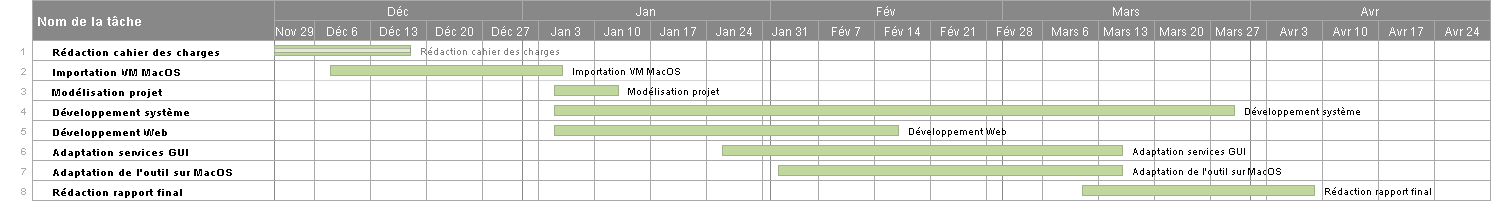
\includegraphics[width=1\textwidth]{../img/gantt.png}
	
	\subsection{Répartition des tâches et moyens humains}
	Afin de mener au mieux ce projet, de simplifier l'organisation et de permettre à tous les membre de la PaquiTeam d'exprimer au mieux ses compétences nous avons décidé de nous répartir les rôles de la manière suivante :
	\begin{itemize}\renewcommand{\labelitemi}{$\bullet$}
		\item Lucas \textsc{Robin} : chef de projet et responsable système, il s'occupera de gérer l'équipe et de garder un \oe{}il sur le bon avancement du projet. En tant que responsable système il devra aussi fournir des informations aux autres membres de l'équipe pour qu'ils comprennent mieux le fonctionnement du système de package et devra s'occuper de la conception du système de création de package;
		\item Kevin \textsc{Fleuriot} : responsable documentation, il devra s'assurer que toutes les fonctionnalités implémentés sont bien documentés et devra s'occuper de la création d'une documentation cohérente et claire;
		\item Alexandre \textsc{Noiret} : Responsable web, il devra designer l'application web permettant d'utiliser Paquito et coordonner son développement;
		\item Yassine \textsc{Ait Elmouden} et Seynabou \textsc{Ka} : experts PHP, ils devront mettre leur expertise en PHP ainsi que leurs connaissance avancée des frameworks utilisés au service de toute l'équipe lors des phases dévelop\-pement et de d'élaboration.
	\end{itemize}
	
	Mais tout ces rôles ont avant tout pour but de structurer le travail. Il ne sont pas exclusifs, et ne veulent en rien dire qu'un des membres de notre équipe devra uniquement s'adonner à sa responsabilité, ni qu'il ne pourra être aidé par une autre personne.

\end{document}
